\subsection{Tipo de entidad Alumno}

   \begin{description}

   \item[Definición] Se refiere a la persona del mundo real: \emph{``Estudiante
        de una titulación que recibe asesoría''}.

   \item[Características] La entidad presenta las siguientes características:
      \begin{itemize}
         \item \textbf{Nombre:} Alumno.
         \item \textbf{Tipo:} Fuerte.
         \item \textbf{Número de atributos:} 19.
         \item \textbf{Atributo/s identificador/es principal/es:} dni\_pasaporte.
         \item \textbf{Atributo/s identificador/es alternativo/s:} correo\_electrónico.
         \item \textbf{Atributo/s heredado/s:} -
      \end{itemize}

   \item[Diagrama] La figura \ref{diagramaAlumno} muestra el diagrama de la entidad.
   \item \begin{figure}[!ht]
            \begin{center}
            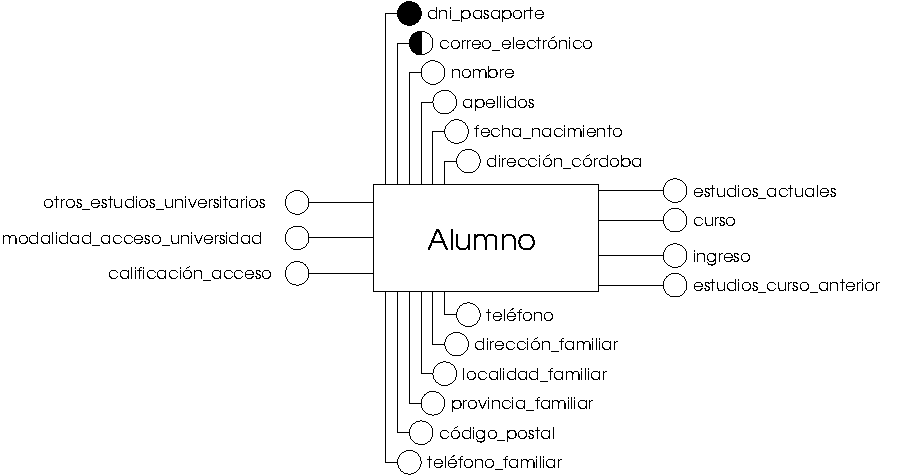
\includegraphics[]{07.Modelo_Entidad-Interrelacion/7.2.Analisis_Entidades/diagramas/alumno.pdf}
            \caption{Diagrama de la entidad Alumno.}
            \label{diagramaAlumno}
            \end{center}
         \end{figure}

   \item[Descripción de los atributos] La entidad presenta los siguientes
   atributos:

   \begin{itemize}
   \item \textbf{dni\_pasaporte}
      \begin{itemize}
         \item \textbf{Definición:} Coincide con el número de documento nacional
         de identidad o pasaporte del alumno.
         \item \textbf{Dominio:} Conjunto de caracteres alfanuméricos.
         \item \textbf{Carácter:} Obligatorio.
         \item \textbf{Ejemplo práctico:} 01234567A.
         \item \textbf{Información adicional:} El dato lo proporciona el usuario alumno, bien a la hora de registrarse, o bien cuando cuando modifica su información personal. Es la clave primaria.
      \end{itemize}
   \item \textbf{correo\_electrónico}
      \begin{itemize}
         \item \textbf{Definición:} Contiene la dirección de correo electrónico de la persona.
         \item \textbf{Dominio:} Conjunto de caracteres alfanuméricos permitidos en una dirección de correo electrónico.
         \item \textbf{Carácter:} Obligatorio.
         \item \textbf{Ejemplo práctico:} i42sasab@uco.es
         \item \textbf{Información adicional:} El dato lo proporciona el usuario alumno cuando se registra o cuando modifica su información personal. Es la clave alterna.
      \end{itemize}
   \item \textbf{nombre}
      \begin{itemize}
         \item \textbf{Definición:} Designa el nombre de pila del usuario alumno que interviene en el sistema.
         \item \textbf{Dominio:} Conjunto de caracteres alfanuméricos.
         \item \textbf{Carácter:} Obligatorio.
         \item \textbf{Ejemplo práctico:} Bartolomé.
         \item \textbf{Información adicional:} El dato lo proporciona el usuario alumno cuando se registra o cuando modifica su información personal.
      \end{itemize}
   \item \textbf{apellidos}
      \begin{itemize}
         \item \textbf{Definición:} Hace referencia a los apellidos del usuario alumno que interviene en el sistema.
         \item \textbf{Dominio:} Conjunto de caracteres alfanuméricos.
         \item \textbf{Carácter:}  Obligatorio.
         \item \textbf{Ejemplo práctico:} Sánchez Salado.
         \item \textbf{Información adicional:} El dato lo proporciona el usuario alumno cuando se registra o cuando modifica su información personal.
      \end{itemize}
   \item \textbf{fecha\_nacimiento}
      \begin{itemize}
         \item \textbf{Definición:} Contiene la fecha de nacimiento del alumno.
         \item \textbf{Dominio:} Formato de fecha: dd-mm-aaaa.
         \item \textbf{Carácter:}  Opcional.
         \item \textbf{Ejemplo práctico:} 13-12-1984.
         \item \textbf{Información adicional:} El dato lo proporciona el usuario alumno cuando se registra o cuando modifica su información personal.
      \end{itemize}
   \item \textbf{dirección\_córdoba}
      \begin{itemize}
         \item \textbf{Definición:} Hace referencia a la dirección del alumno durante el curso.
         \item \textbf{Dominio:} Conjunto de caracteres alfanuméricos.
         \item \textbf{Carácter:}  Opcional.
         \item \textbf{Ejemplo práctico:} 13 Rue del Percebe.
         \item \textbf{Información adicional:} El dato lo proporciona el usuario alumno cuando se registra o cuando modifica su información personal.
      \end{itemize}
   \item \textbf{teléfono}
      \begin{itemize}
         \item \textbf{Definición:} Hace referencia a un número de teléfono perteneciente al alumno.
         \item \textbf{Dominio:} Conjunto de enteros positivos.
         \item \textbf{Carácter:}  Opcional.
         \item \textbf{Ejemplo práctico:} 601234567.
         \item \textbf{Información adicional:} El dato lo proporciona el usuario alumno cuando se registra o cuando modifica su información personal.
      \end{itemize}
   \item \textbf{dirección\_familiar}
      \begin{itemize}
         \item \textbf{Definición:} Hace referencia a la dirección del domicilio familiar del alumno.
         \item \textbf{Dominio:} Conjunto de caracteres alfanuméricos.
         \item \textbf{Carácter:}  Opcional.
         \item \textbf{Ejemplo práctico:} Calle Edsger Dijkstra, 30.
         \item \textbf{Información adicional:} El dato lo proporciona el usuario alumno cuando se registra o cuando modifica su información personal.
      \end{itemize}
   \item \textbf{localidad\_familiar}
      \begin{itemize}
         \item \textbf{Definición:} Hace referencia a la localidad del domicilio familiar del alumno.
         \item \textbf{Dominio:} Conjunto de caracteres alfanuméricos.
         \item \textbf{Carácter:}  Opcional.
         \item \textbf{Ejemplo práctico:} La Carlota.
         \item \textbf{Información adicional:} El dato lo proporciona el usuario alumno cuando se registra o cuando modifica su información personal.
      \end{itemize}
   \item \textbf{provincia\_familiar}
      \begin{itemize}
         \item \textbf{Definición:} Hace referencia a la provincia del domicilio familiar del alumno.
         \item \textbf{Dominio:} Conjunto de caracteres alfanuméricos.
         \item \textbf{Carácter:}  Opcional.
         \item \textbf{Ejemplo práctico:} Córdoba.
         \item \textbf{Información adicional:} El dato lo proporciona el usuario alumno cuando se registra o cuando modifica su información personal.
      \end{itemize}
   \item \textbf{código\_postal}
      \begin{itemize}
         \item \textbf{Definición:} Hace referencia al código postal de la localidad del domicilio familiar del alumno.
         \item \textbf{Dominio:} Conjunto de caracteres alfanuméricos.
         \item \textbf{Carácter:}  Opcional.
         \item \textbf{Ejemplo práctico:} 14100.
         \item \textbf{Información adicional:} El dato lo proporciona el usuario alumno cuando se registra o cuando modifica su información personal.
      \end{itemize}
   \item \textbf{teléfono\_familiar}
      \begin{itemize}
         \item \textbf{Definición:} Hace referencia al número de teléfono del domicilio familiar del alumno.
         \item \textbf{Dominio:} Conjunto de enteros positivos.
         \item \textbf{Carácter:}  Opcional.
         \item \textbf{Ejemplo práctico:} 957123456.
         \item \textbf{Información adicional:} El dato lo proporciona el usuario alumno cuando se registra o cuando modifica su información personal.
      \end{itemize}
   \item \textbf{ingreso}
      \begin{itemize}
         \item \textbf{Definición:} Hace referencia al año de ingreso en la Universidad por parte del alumno en sus estudios actuales.
         \item \textbf{Dominio:} Formato de fecha: aaaa.
         \item \textbf{Carácter:}  Opcional.
         \item \textbf{Ejemplo práctico:} 2004.
         \item \textbf{Información adicional:} El dato lo proporciona el usuario alumno cuando se registra o cuando modifica su información personal.
      \end{itemize}
   \item \textbf{otros\_estudios\_universitarios}
      \begin{itemize}
         \item \textbf{Definición:} Hace referencia a otros estudios universitarios que posea el alumno.
         \item \textbf{Dominio:} Conjunto de caracteres alfanuméricos.
         \item \textbf{Carácter:}  Opcional.
         \item \textbf{Ejemplo práctico:} -
         \item \textbf{Información adicional:} El dato lo proporciona el usuario alumno cuando se registra o cuando modifica su información personal. Se trata de un atributo múltiple.
      \end{itemize}
   \item \textbf{modalidad\_acceso\_universidad}
      \begin{itemize}
         \item \textbf{Definición:} Hace referencia al modo en que el alumno accedió a la Universidad.
         \item \textbf{Dominio:} Conjunto de caracteres alfanuméricos.
         \item \textbf{Carácter:}  Opcional.
         \item \textbf{Ejemplo práctico:} Selectividad.
         \item \textbf{Información adicional:} El dato lo proporciona el usuario alumno cuando se registra o cuando modifica su información personal.
      \end{itemize}
   \item \textbf{calificación\_acceso}
      \begin{itemize}
         \item \textbf{Definición:} Hace referencia a la calificación obtenida en las distintas modalidades de acceso a la Universidad por parte del alumno.
         \item \textbf{Dominio:} Conjunto de reales positivos.
         \item \textbf{Carácter:}  Opcional.
         \item \textbf{Ejemplo práctico:} 7.2.
         \item \textbf{Información adicional:} El dato lo proporciona el usuario alumno cuando se registra o cuando modifica su información personal.
      \end{itemize}
   \end{itemize}

   \item[Ejemplo práctico]

   \item \begin{center}
            \begin{tabular}{ | l | l | }
            \hline
            \multicolumn{2}{ | c | }{\textbf{Tipo de entidad Alumno}} \\
            \hline
            dni\_pasaporte & 01234567A \\
            \hline
            correo\_electrónico & i42sasab@uco.es\\
            \hline
            nombre & Bartolomé\\
            \hline
            apellidos & Sánchez Salado\\
            \hline
            fecha\_nacimiento & 1984\\
            \hline
            dirección\_córdoba & 13 Rue del Percebe\\
            \hline
            teléfono & 601234567\\
            \hline
            dirección\_familiar & Calle Edsger Dijkstra, 30\\
            \hline
            localidad\_familiar & La Carlota\\
            \hline
            provincia\_familiar & Córdoba\\
            \hline
            código\_postal & 14100\\
            \hline
            teléfono\_familiar & 957123456\\
            \hline
            ingreso & 2004\\
            \hline
            otros\_estudios\_universitarios & -\\
            \hline
            modalidad\_acceso\_universidad & Selectividad\\
            \hline
            calificación\_acceso & 7.2\\
            \hline
            \end{tabular}
         \end{center}
   \end{description}
